\chapter{Deterministic Chaos vs. Stochastic Turbulence}
\label{c_chaos}

\section{Lorentzian Pulses as an Indicator of Chaos}
\label{s_lorentzian_pulses}


Here, I revisit the time signals and the frequency spectra of the density and $I_{sat}$ signals to connect the simulations and the experiment to some recent theoretical findings. 
Now, typically, people do not compare time signals of chaotic systems because the sensitivity
to initial conditions ensures that time signals of different experiments or simulations will certainly not be identical, and any qualitative judgements are too subjective. On the other hand,
strange attractors do sometimes have properties with identifiable visual characteristics. For example, the orbits of the well-known Lorenz attractor look like the wings of a butterfly~\cite{lorenz1963}.
Recently, Pace et al. discovered that the time signals in some LAPD experiments and in the edge of some magnetic confinement devices
are made up of Lorentzian-shaped pulses~\cite{pace2008a,pace2008b}. A Lorentzian is simply a function of the form

\beq
\label{lorentz_eqn}
f(t) = A/\left[1 + (t - t_0)^2/\tau^2 \right]
\eeq
where $A$ is the pulse amplitude, $t_0$ is its center, and $\tau$ is the pulse width. Now since the absolute value of the Fourier transform of a Lorentzian is simply a decaying exponential,
the Lorentzian pulses in the time signals lead to frequency power spectra that have exponential shape, which show up as a straight line in a log-linear plot. In such a plot, the slope of the line
is proportional to the Lorentzian width $\tau$. Sometimes, however, the Lorentzian
pulses in the time signals have different widths, which cause different spectral slopes, leading to power spectra with non-exponential shape. 

To explore this finding in the experiment that I have described in this Chapter as well as in the simulations, I plot the frequency spectra of the experiment,
the Periodic simulation, and the $n=0$ suppressed simulation in Fig.~\ref{lorentzians} a). I don't use any window functions, since they could distort any structures in the time signals,
and I use only one radial location (30 cm) rather than doing a volume average. Clearly, the spectra are not exponential for either the experiment or the simulations. This doesn't rule out
Lorentzian pulses in the time signals, however, as long as the time signals have pulses of varying width. So next, I look at the time signals of the experiment and simulations. I show representative
signals for the experiment, Periodic simulation, and $n=0$ suppressed simulation in Figs.~\ref{lorentzians} b), c), and d), respectively. Notice that the experiment and Periodic simulation
appear to have qualitatively similar time signals, while the $n=0$ suppressed simulation has a much different, simpler looking signal. Furthermore, the experiment and Periodic simulation contain
a number of pulse-like features. I take a closer look at some of these pulses in Figs.~\ref{lorentzians} e) (experiment) and f) (Periodic simulation), trying to find times when the pulses
are relatively isolated. In Fig.~\ref{lorentzians} e), I fit one of these pulses to a Lorentzian function (the dashed line), 
proving that this pulse, does in fact have a Lorentzian shape. I confirm that a Lorentzian does provide a better fit than a Gaussian, which doesn't fit the pulse as well for as long of a time
range as the Lorentzian. Furthermore, Gaussian pulses create spectra that look very different from those in Fig.~\ref{lorentzians} a), supporting the claim that the pulses have Lorentzian
shape rather than Gaussian. Finally, in Fig.~\ref{lorentzians} f),
I look at a signal snipet from the Periodic simulation with two relatively isolated pulses, and I fit a sum of two Lorentzian functions to this. Clearly, the fit is excellent as
both of these pulses have Lorentzian shape, and importantly, they have different widths, explaining the non-exponential shape of the spectra. I don't show a fit to the $n=0$ suppressed simulation
signal, but I note that it is quite sinusoidal with seemingly two or so dominant low frequency waves, which is clear from the highly peaked, non-broadband frequency spectra.

\begin{figure}[!ht]
\centerline{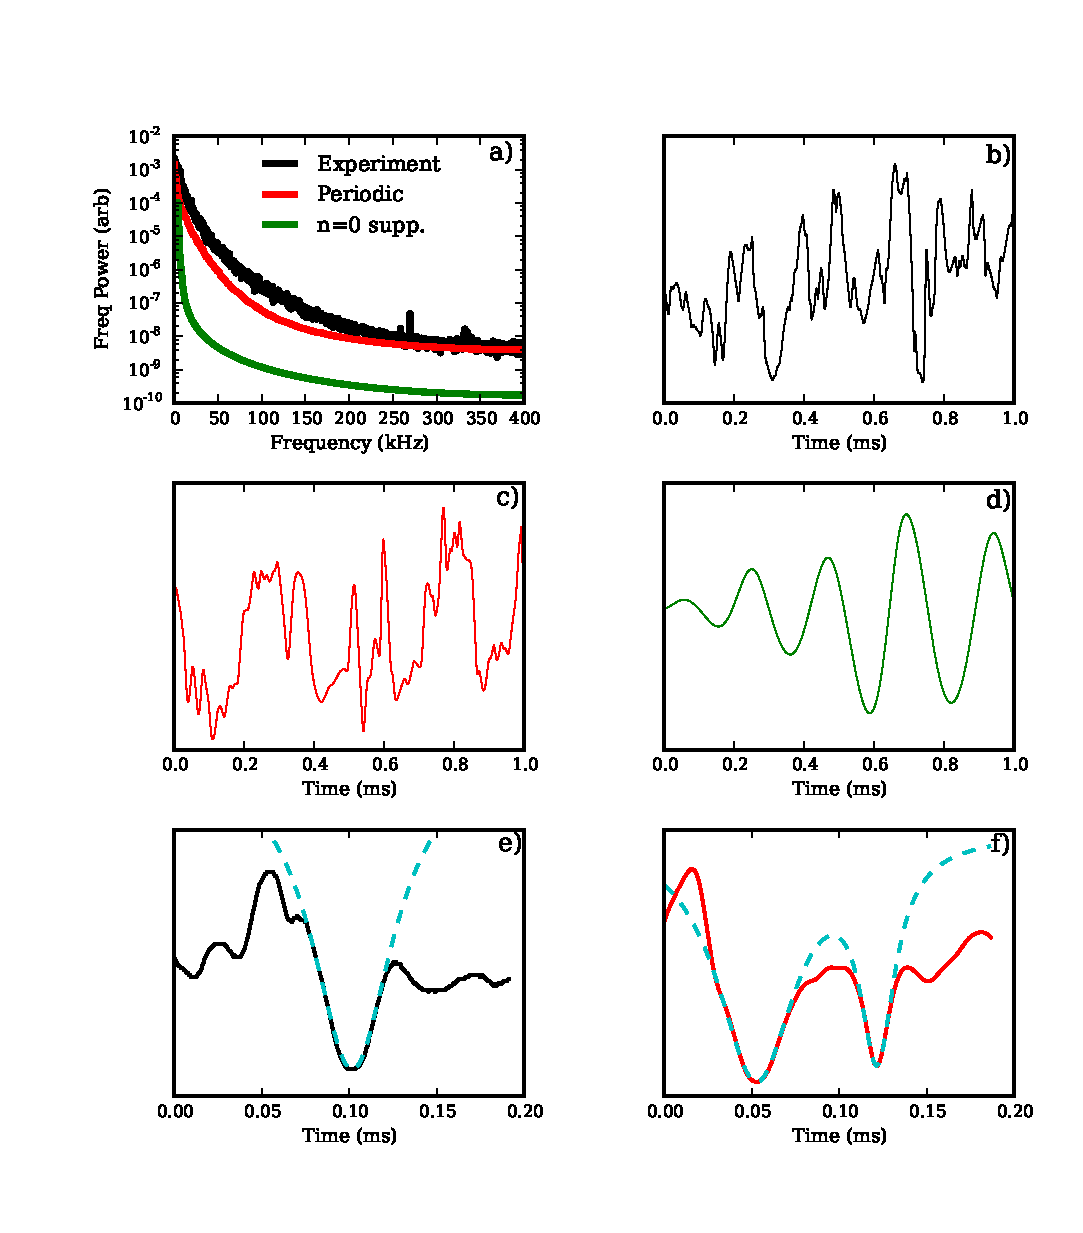
\includegraphics[]{lorentzians}}
\caption{Lorentzian pulses in time signals}
\label{lorentzians}
\end{figure}

Now the reason for the Lorentzian pulses in the time signals was explained by Maggs and Morales~\cite{maggs2012a}. They showed that in nonlinear systems, 
right around the bifurcation from limit cycle attractors to chaotic strange attractors, one of the variables has a trajectory that involves a Lorentzian pulse or a series of Lorentzian pulses.
In a plasma, that trajectory is associated with an ${\bf E \times B}$ flow, which advects the scalar density and temperature, imprinting the Lorentzian shape onto them.
The fact that experimental signals are made up of Lorentzian pulses indicates that the systems are deterministic, not random, and they are associated with the mathematical construct called
a strange attractor. Furthermore, these systems have some control parameter or bifurcation parameter associated with them that determines their steady state, 
like how nuetral fluids have the Reynolds number which partially determines the attractor into which the system falls. For LAPD and similar plasma systems, the control parameter should be
proportional to the equilibrium gradients. Then, for the system to display Lorentzian chaotic dynamics, the control parameter and thus the gradient must be high enough so that the attractor is not
still a limit cycle, but low enough so that the attractor still has a Lorentzian trajectory associated with it.
The fact that both the simulation and the experiment have Lorentzian trajectories means that both are governed by a nonlinear deterministic chaotic process where their bifurcation parameters
are just above the limit cycle threashold. This lends further support to the validation of the simulation model. The fact that the control parameter is not too far above the chaotic bifurcation
should not be surprising because once chaos ensues, transport occurs, which relaxes the gradients or prevents them from building up. Therefore, the chaos regulates the control parameter,
preventing further bifurcation to a more stochastic state.

\section{Entropy and Complexity as an Indicator of Chaos}
\label{s_ent_comp}

\begin{figure}[!ht]
\centerline{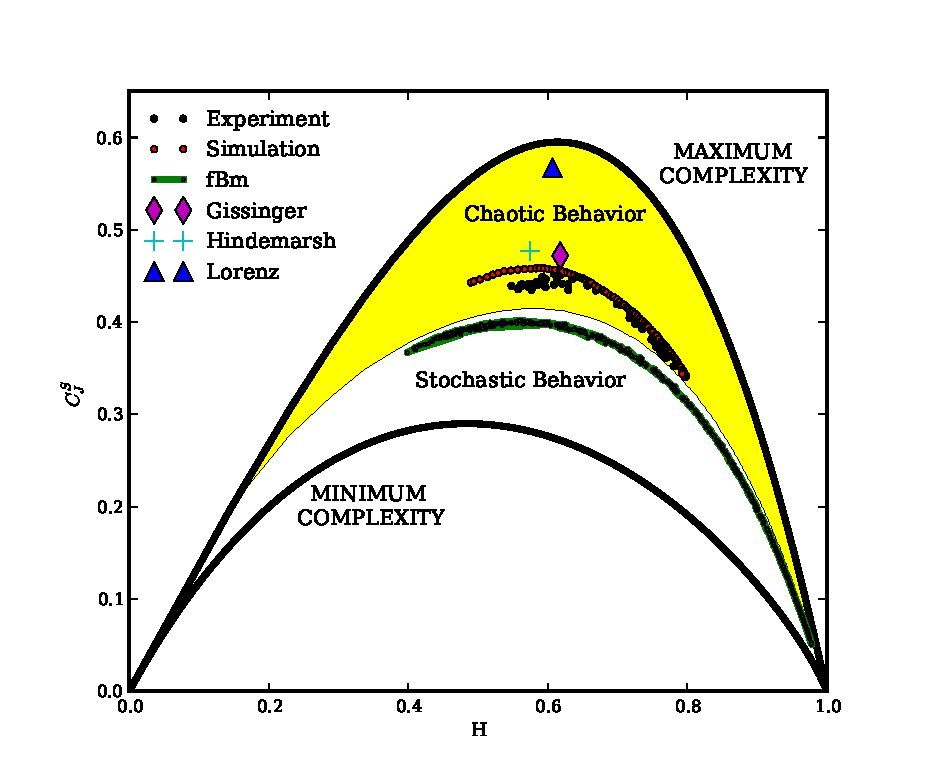
\includegraphics[]{entropy_complexity}}
\caption{Entropy-complexity results for Bandt-Pompe distribution functions}
\label{entropy_complexity}
\end{figure}
